% Options for packages loaded elsewhere
\PassOptionsToPackage{unicode}{hyperref}
\PassOptionsToPackage{hyphens}{url}
%
\documentclass[
]{article}
\usepackage{lmodern}
\usepackage{amssymb,amsmath}
\usepackage{ifxetex,ifluatex}
\ifnum 0\ifxetex 1\fi\ifluatex 1\fi=0 % if pdftex
  \usepackage[T1]{fontenc}
  \usepackage[utf8]{inputenc}
  \usepackage{textcomp} % provide euro and other symbols
\else % if luatex or xetex
  \usepackage{unicode-math}
  \defaultfontfeatures{Scale=MatchLowercase}
  \defaultfontfeatures[\rmfamily]{Ligatures=TeX,Scale=1}
\fi
% Use upquote if available, for straight quotes in verbatim environments
\IfFileExists{upquote.sty}{\usepackage{upquote}}{}
\IfFileExists{microtype.sty}{% use microtype if available
  \usepackage[]{microtype}
  \UseMicrotypeSet[protrusion]{basicmath} % disable protrusion for tt fonts
}{}
\makeatletter
\@ifundefined{KOMAClassName}{% if non-KOMA class
  \IfFileExists{parskip.sty}{%
    \usepackage{parskip}
  }{% else
    \setlength{\parindent}{0pt}
    \setlength{\parskip}{6pt plus 2pt minus 1pt}}
}{% if KOMA class
  \KOMAoptions{parskip=half}}
\makeatother
\usepackage{xcolor}
\IfFileExists{xurl.sty}{\usepackage{xurl}}{} % add URL line breaks if available
\IfFileExists{bookmark.sty}{\usepackage{bookmark}}{\usepackage{hyperref}}
\hypersetup{
  pdftitle={Results of PangoVis},
  pdfauthor={Devan Becker},
  hidelinks,
  pdfcreator={LaTeX via pandoc}}
\urlstyle{same} % disable monospaced font for URLs
\usepackage[margin=1in]{geometry}
\usepackage{color}
\usepackage{fancyvrb}
\newcommand{\VerbBar}{|}
\newcommand{\VERB}{\Verb[commandchars=\\\{\}]}
\DefineVerbatimEnvironment{Highlighting}{Verbatim}{commandchars=\\\{\}}
% Add ',fontsize=\small' for more characters per line
\usepackage{framed}
\definecolor{shadecolor}{RGB}{248,248,248}
\newenvironment{Shaded}{\begin{snugshade}}{\end{snugshade}}
\newcommand{\AlertTok}[1]{\textcolor[rgb]{0.94,0.16,0.16}{#1}}
\newcommand{\AnnotationTok}[1]{\textcolor[rgb]{0.56,0.35,0.01}{\textbf{\textit{#1}}}}
\newcommand{\AttributeTok}[1]{\textcolor[rgb]{0.77,0.63,0.00}{#1}}
\newcommand{\BaseNTok}[1]{\textcolor[rgb]{0.00,0.00,0.81}{#1}}
\newcommand{\BuiltInTok}[1]{#1}
\newcommand{\CharTok}[1]{\textcolor[rgb]{0.31,0.60,0.02}{#1}}
\newcommand{\CommentTok}[1]{\textcolor[rgb]{0.56,0.35,0.01}{\textit{#1}}}
\newcommand{\CommentVarTok}[1]{\textcolor[rgb]{0.56,0.35,0.01}{\textbf{\textit{#1}}}}
\newcommand{\ConstantTok}[1]{\textcolor[rgb]{0.00,0.00,0.00}{#1}}
\newcommand{\ControlFlowTok}[1]{\textcolor[rgb]{0.13,0.29,0.53}{\textbf{#1}}}
\newcommand{\DataTypeTok}[1]{\textcolor[rgb]{0.13,0.29,0.53}{#1}}
\newcommand{\DecValTok}[1]{\textcolor[rgb]{0.00,0.00,0.81}{#1}}
\newcommand{\DocumentationTok}[1]{\textcolor[rgb]{0.56,0.35,0.01}{\textbf{\textit{#1}}}}
\newcommand{\ErrorTok}[1]{\textcolor[rgb]{0.64,0.00,0.00}{\textbf{#1}}}
\newcommand{\ExtensionTok}[1]{#1}
\newcommand{\FloatTok}[1]{\textcolor[rgb]{0.00,0.00,0.81}{#1}}
\newcommand{\FunctionTok}[1]{\textcolor[rgb]{0.00,0.00,0.00}{#1}}
\newcommand{\ImportTok}[1]{#1}
\newcommand{\InformationTok}[1]{\textcolor[rgb]{0.56,0.35,0.01}{\textbf{\textit{#1}}}}
\newcommand{\KeywordTok}[1]{\textcolor[rgb]{0.13,0.29,0.53}{\textbf{#1}}}
\newcommand{\NormalTok}[1]{#1}
\newcommand{\OperatorTok}[1]{\textcolor[rgb]{0.81,0.36,0.00}{\textbf{#1}}}
\newcommand{\OtherTok}[1]{\textcolor[rgb]{0.56,0.35,0.01}{#1}}
\newcommand{\PreprocessorTok}[1]{\textcolor[rgb]{0.56,0.35,0.01}{\textit{#1}}}
\newcommand{\RegionMarkerTok}[1]{#1}
\newcommand{\SpecialCharTok}[1]{\textcolor[rgb]{0.00,0.00,0.00}{#1}}
\newcommand{\SpecialStringTok}[1]{\textcolor[rgb]{0.31,0.60,0.02}{#1}}
\newcommand{\StringTok}[1]{\textcolor[rgb]{0.31,0.60,0.02}{#1}}
\newcommand{\VariableTok}[1]{\textcolor[rgb]{0.00,0.00,0.00}{#1}}
\newcommand{\VerbatimStringTok}[1]{\textcolor[rgb]{0.31,0.60,0.02}{#1}}
\newcommand{\WarningTok}[1]{\textcolor[rgb]{0.56,0.35,0.01}{\textbf{\textit{#1}}}}
\usepackage{longtable,booktabs}
% Correct order of tables after \paragraph or \subparagraph
\usepackage{etoolbox}
\makeatletter
\patchcmd\longtable{\par}{\if@noskipsec\mbox{}\fi\par}{}{}
\makeatother
% Allow footnotes in longtable head/foot
\IfFileExists{footnotehyper.sty}{\usepackage{footnotehyper}}{\usepackage{footnote}}
\makesavenoteenv{longtable}
\usepackage{graphicx}
\makeatletter
\def\maxwidth{\ifdim\Gin@nat@width>\linewidth\linewidth\else\Gin@nat@width\fi}
\def\maxheight{\ifdim\Gin@nat@height>\textheight\textheight\else\Gin@nat@height\fi}
\makeatother
% Scale images if necessary, so that they will not overflow the page
% margins by default, and it is still possible to overwrite the defaults
% using explicit options in \includegraphics[width, height, ...]{}
\setkeys{Gin}{width=\maxwidth,height=\maxheight,keepaspectratio}
% Set default figure placement to htbp
\makeatletter
\def\fps@figure{htbp}
\makeatother
\setlength{\emergencystretch}{3em} % prevent overfull lines
\providecommand{\tightlist}{%
  \setlength{\itemsep}{0pt}\setlength{\parskip}{0pt}}
\setcounter{secnumdepth}{-\maxdimen} % remove section numbering
\usepackage[]{natbib}
\bibliographystyle{plainnat}

\title{Results of PangoVis}
\author{Devan Becker}
\date{2021-04-15}

\begin{document}
\maketitle

\hypertarget{load-packages-and-data}{%
\section{Load Packages and Data}\label{load-packages-and-data}}

\begin{Shaded}
\begin{Highlighting}[]
\CommentTok{\# Packages that Art hates}
\KeywordTok{library}\NormalTok{(dplyr)}
\KeywordTok{library}\NormalTok{(tidyr)}
\KeywordTok{library}\NormalTok{(ggplot2)}
\KeywordTok{library}\NormalTok{(stringr)}
\KeywordTok{library}\NormalTok{(here)}

\NormalTok{dirich \textless{}{-}}\StringTok{ }\NormalTok{params}\OperatorTok{$}\NormalTok{dirich}

\CommentTok{\# Read in CSV files}
\NormalTok{csvs \textless{}{-}}\StringTok{ }\KeywordTok{list.files}\NormalTok{(}\KeywordTok{here}\NormalTok{(}\StringTok{"data/"}\NormalTok{, }\StringTok{"pangolineages"}\NormalTok{),}
    \DataTypeTok{pattern =} \KeywordTok{ifelse}\NormalTok{(dirich, }\StringTok{"*\_d.csv"}\NormalTok{, }\StringTok{"*.csv"}\NormalTok{),}
    \DataTypeTok{full.names =} \OtherTok{TRUE}\NormalTok{)}

\CommentTok{\# Remove any copies}
\NormalTok{csvs \textless{}{-}}\StringTok{ }\NormalTok{csvs[}\OperatorTok{!}\KeywordTok{grepl}\NormalTok{(}\StringTok{"{-}1"}\NormalTok{, csvs)]}

\CommentTok{\# Bring them into one data frame}
\NormalTok{lins \textless{}{-}}\StringTok{ }\KeywordTok{bind\_rows}\NormalTok{(}\KeywordTok{lapply}\NormalTok{(csvs, read.csv))}

\CommentTok{\# Taxon is encoded as \_ACCSESSIONNUMBER.ID, split into ACCESSIONNUMBER and ID}
\NormalTok{lins \textless{}{-}}\StringTok{ }\NormalTok{lins }\OperatorTok{\%\textgreater{}\%}
\StringTok{    }\KeywordTok{separate}\NormalTok{(}\DataTypeTok{col =} \StringTok{"taxon"}\NormalTok{, }\DataTypeTok{sep =} \StringTok{"}\CharTok{\textbackslash{}\textbackslash{}}\StringTok{."}\NormalTok{,}
        \DataTypeTok{into =} \KeywordTok{c}\NormalTok{(}\StringTok{"taxon"}\NormalTok{, }\StringTok{"sample"}\NormalTok{)) }\OperatorTok{\%\textgreater{}\%}
\StringTok{    }\KeywordTok{mutate}\NormalTok{(}\DataTypeTok{taxon =} \KeywordTok{str\_replace}\NormalTok{(taxon, }\StringTok{"}\CharTok{\textbackslash{}\textbackslash{}}\StringTok{\_"}\NormalTok{, }\StringTok{""}\NormalTok{))}

\NormalTok{badlins \textless{}{-}}\StringTok{ }\KeywordTok{table}\NormalTok{(lins}\OperatorTok{$}\NormalTok{taxon)}
\NormalTok{badlins \textless{}{-}}\StringTok{ }\KeywordTok{names}\NormalTok{(badlins[}\KeywordTok{which}\NormalTok{(badlins }\OperatorTok{\textless{}}\StringTok{ }\DecValTok{4500}\NormalTok{)])}
\KeywordTok{cat}\NormalTok{(}\KeywordTok{length}\NormalTok{(badlins), }\StringTok{" runs were removed for having too few samples."}\NormalTok{)}
\end{Highlighting}
\end{Shaded}

\begin{verbatim}
## 10  runs were removed for having too few samples.
\end{verbatim}

\begin{Shaded}
\begin{Highlighting}[]
\NormalTok{lins \textless{}{-}}\StringTok{ }\KeywordTok{filter}\NormalTok{(lins, }\OperatorTok{!}\NormalTok{taxon }\OperatorTok{\%in\%}\StringTok{ }\NormalTok{badlins)}

\CommentTok{\#\#\#\# Visualize the uncertainty in the base calls {-}{-}{-}{-}}
\NormalTok{taxons \textless{}{-}}\StringTok{ }\KeywordTok{sort}\NormalTok{(}\KeywordTok{unique}\NormalTok{(lins}\OperatorTok{$}\NormalTok{taxon))}
\KeywordTok{length}\NormalTok{(taxons)}
\end{Highlighting}
\end{Shaded}

\begin{verbatim}
## [1] 138
\end{verbatim}

\hypertarget{abstract-info}{%
\section{Abstract Info}\label{abstract-info}}

\begin{Shaded}
\begin{Highlighting}[]
\NormalTok{summs \textless{}{-}}\StringTok{ }\NormalTok{lins }\OperatorTok{\%\textgreater{}\%}
\StringTok{    }\KeywordTok{group\_by}\NormalTok{(taxon) }\OperatorTok{\%\textgreater{}\%}
\StringTok{    }\KeywordTok{summarise}\NormalTok{(}
        \DataTypeTok{maxperc =} \KeywordTok{mean}\NormalTok{(lineage }\OperatorTok{==}\StringTok{ }\KeywordTok{names}\NormalTok{(}\KeywordTok{sort}\NormalTok{(}\KeywordTok{table}\NormalTok{(lineage),}
            \DataTypeTok{decreasing =} \OtherTok{TRUE}\NormalTok{)[}\DecValTok{1}\NormalTok{])),}
        \DataTypeTok{uniques =} \KeywordTok{length}\NormalTok{(}\KeywordTok{unique}\NormalTok{(lineage)),}
        \DataTypeTok{minpango =} \KeywordTok{min}\NormalTok{(probability),}
        \DataTypeTok{maxpango =} \KeywordTok{max}\NormalTok{(probability),}
        \DataTypeTok{menpango =} \KeywordTok{mean}\NormalTok{(probability),}
        \DataTypeTok{max =} \KeywordTok{names}\NormalTok{(}\KeywordTok{sort}\NormalTok{(}\KeywordTok{table}\NormalTok{(lineage), }\DataTypeTok{decreasing =} \OtherTok{TRUE}\NormalTok{))[}\DecValTok{1}\NormalTok{])}
\end{Highlighting}
\end{Shaded}

\begin{verbatim}
## `summarise()` ungrouping output (override with `.groups` argument)
\end{verbatim}

\begin{Shaded}
\begin{Highlighting}[]
\KeywordTok{print}\NormalTok{(}\StringTok{"summary info"}\NormalTok{)}
\end{Highlighting}
\end{Shaded}

\begin{verbatim}
## [1] "summary info"
\end{verbatim}

\begin{Shaded}
\begin{Highlighting}[]
\KeywordTok{print}\NormalTok{(summs)}
\end{Highlighting}
\end{Shaded}

\begin{verbatim}
## # A tibble: 138 x 7
##    taxon      maxperc uniques minpango maxpango menpango max      
##    <chr>        <dbl>   <int>    <dbl>    <dbl>    <dbl> <chr>    
##  1 ERR4305816   0.958      15        1        1        1 B.3.1    
##  2 ERR4307842   0.950      29        1        1        1 B.1.1.289
##  3 ERR4363387   0.953      27        1        1        1 B.1.222  
##  4 ERR4364007   0.855      89        1        1        1 B.1.1.29 
##  5 ERR4440194   0.515      18        1        1        1 B.1      
##  6 ERR4440219   0.937      70        1        1        1 B.1.1.164
##  7 ERR4440247   0.631     227        1        1        1 B.1.1.29 
##  8 ERR4440332   0.984       8        1        1        1 B.40     
##  9 ERR4440354   0.665     211        1        1        1 B.1.1.29 
## 10 ERR4440373   0.995       9        1        1        1 B.40     
## # ... with 128 more rows
\end{verbatim}

\begin{Shaded}
\begin{Highlighting}[]
\DecValTok{1} \OperatorTok{{-}}\StringTok{ }\KeywordTok{mean}\NormalTok{(summs}\OperatorTok{$}\NormalTok{maxperc); }\DecValTok{1} \OperatorTok{{-}}\StringTok{ }\KeywordTok{mean}\NormalTok{(summs}\OperatorTok{$}\NormalTok{menpango)}
\end{Highlighting}
\end{Shaded}

\begin{verbatim}
## [1] 0.1098993
\end{verbatim}

\begin{verbatim}
## [1] 0.03622898
\end{verbatim}

\hypertarget{stacked-bar-plots}{%
\section{Stacked Bar Plots}\label{stacked-bar-plots}}

\scriptsize

\begin{Shaded}
\begin{Highlighting}[]
\NormalTok{max\_label \textless{}{-}}\StringTok{ }\DecValTok{250}
\NormalTok{other\_label \textless{}{-}}\StringTok{ }\DecValTok{100}

\KeywordTok{par}\NormalTok{(}\DataTypeTok{mfrow =} \KeywordTok{c}\NormalTok{(}\DecValTok{17}\NormalTok{, }\DecValTok{1}\NormalTok{), }\DataTypeTok{mar =} \KeywordTok{c}\NormalTok{(}\FloatTok{0.05}\NormalTok{, }\FloatTok{7.75}\NormalTok{, }\FloatTok{0.05}\NormalTok{, }\FloatTok{0.05}\NormalTok{))}
\ControlFlowTok{if}\NormalTok{ (}\KeywordTok{exists}\NormalTok{(}\StringTok{"seq\_info"}\NormalTok{)) }\KeywordTok{rm}\NormalTok{(seq\_info)}
\ControlFlowTok{for}\NormalTok{ (i }\ControlFlowTok{in} \KeywordTok{seq\_along}\NormalTok{(taxons)) \{}
\NormalTok{    pang \textless{}{-}}\StringTok{ }\NormalTok{lins[lins}\OperatorTok{$}\NormalTok{taxon }\OperatorTok{==}\StringTok{ }\NormalTok{taxons[i], ]}
\NormalTok{    called \textless{}{-}}\StringTok{ }\NormalTok{pang}\OperatorTok{$}\NormalTok{lineage[pang}\OperatorTok{$}\NormalTok{sample }\OperatorTok{==}\StringTok{ }\DecValTok{0}\NormalTok{][}\DecValTok{1}\NormalTok{]}
\NormalTok{    pangtab \textless{}{-}}\StringTok{ }\KeywordTok{sort}\NormalTok{(}\KeywordTok{table}\NormalTok{(pang}\OperatorTok{$}\NormalTok{lineage), }\DataTypeTok{decreasing =} \OtherTok{TRUE}\NormalTok{)}

    \CommentTok{\# Prep the data for a nicely formatted table}
    \CommentTok{\# Subtract one because of the conseq.}
\NormalTok{    seq\_info\_i \textless{}{-}}\StringTok{ }\KeywordTok{data.frame}\NormalTok{(}
        \DataTypeTok{called =}\NormalTok{ called,}
        \DataTypeTok{mode =} \KeywordTok{names}\NormalTok{(pangtab)[}\DecValTok{1}\NormalTok{],}
            \DataTypeTok{mode\_n =}\NormalTok{ pangtab[}\DecValTok{1}\NormalTok{] }\OperatorTok{{-}}\StringTok{ }\DecValTok{1}\NormalTok{,}
            \DataTypeTok{perc =} \KeywordTok{round}\NormalTok{(}\DecValTok{100} \OperatorTok{*}\StringTok{ }\NormalTok{(pangtab[}\DecValTok{1}\NormalTok{] }\OperatorTok{{-}}\StringTok{ }\DecValTok{1}\NormalTok{) }\OperatorTok{/}\StringTok{ }\NormalTok{(}\KeywordTok{sum}\NormalTok{(pangtab) }\OperatorTok{{-}}\StringTok{ }\DecValTok{1}\NormalTok{), }\DecValTok{2}\NormalTok{),}
        \DataTypeTok{runner\_up =} \KeywordTok{names}\NormalTok{(pangtab)[}\DecValTok{2}\NormalTok{],}
            \DataTypeTok{ru\_n =}\NormalTok{ pangtab[}\DecValTok{2}\NormalTok{],}
        \DataTypeTok{unique =} \KeywordTok{length}\NormalTok{(pangtab), }\DataTypeTok{atoms =} \KeywordTok{sum}\NormalTok{(pangtab }\OperatorTok{==}\StringTok{ }\DecValTok{1}\NormalTok{))}
\NormalTok{    seq\_info\_i}\OperatorTok{$}\NormalTok{taxon \textless{}{-}}\StringTok{ }\NormalTok{taxons[i]}

    \ControlFlowTok{if}\NormalTok{ (}\OperatorTok{!}\KeywordTok{exists}\NormalTok{(}\StringTok{"seq\_info"}\NormalTok{)) \{}
\NormalTok{        seq\_info \textless{}{-}}\StringTok{ }\NormalTok{seq\_info\_i}
\NormalTok{    \} }\ControlFlowTok{else}\NormalTok{ \{}
\NormalTok{        seq\_info \textless{}{-}}\StringTok{ }\KeywordTok{bind\_rows}\NormalTok{(seq\_info, seq\_info\_i)}
\NormalTok{    \}}

\NormalTok{    colvec \textless{}{-}}\StringTok{ }\KeywordTok{rep}\NormalTok{(}\StringTok{"grey"}\NormalTok{, }\KeywordTok{length}\NormalTok{(pangtab))}
\NormalTok{    colvec[}\KeywordTok{which}\NormalTok{(}\KeywordTok{names}\NormalTok{(pangtab) }\OperatorTok{==}\StringTok{ }\NormalTok{called)] \textless{}{-}}\StringTok{ "red"}

\NormalTok{    n \textless{}{-}}\StringTok{ }\KeywordTok{sum}\NormalTok{(pangtab }\OperatorTok{\textgreater{}}\StringTok{ }\NormalTok{max\_label)}
    \ControlFlowTok{if}\NormalTok{ (n }\OperatorTok{\textgreater{}}\StringTok{ }\DecValTok{1}\NormalTok{) \{}
\NormalTok{        add\_other \textless{}{-}}\StringTok{ }\OtherTok{FALSE}
        \ControlFlowTok{if}\NormalTok{ (}\KeywordTok{sum}\NormalTok{(pangtab }\OperatorTok{\textless{}}\StringTok{ }\NormalTok{other\_label) }\OperatorTok{\textgreater{}}\StringTok{ }\DecValTok{10}\NormalTok{) \{}
\NormalTok{            add\_other \textless{}{-}}\StringTok{ }\OtherTok{TRUE}
\NormalTok{            other\_count \textless{}{-}}\StringTok{ }\KeywordTok{sum}\NormalTok{(pangtab }\OperatorTok{\textless{}=}\StringTok{ }\NormalTok{other\_label)}
\NormalTok{            pangtab \textless{}{-}}\StringTok{ }\KeywordTok{c}\NormalTok{(pangtab[pangtab }\OperatorTok{\textgreater{}}\StringTok{ }\NormalTok{other\_label],}
                \KeywordTok{c}\NormalTok{(}\StringTok{"other"}\NormalTok{ =}\StringTok{ }\KeywordTok{sum}\NormalTok{(pangtab[pangtab }\OperatorTok{\textless{}=}\StringTok{ }\NormalTok{other\_label])))}
\NormalTok{            colvec[}\KeywordTok{which}\NormalTok{(}\KeywordTok{names}\NormalTok{(pangtab) }\OperatorTok{==}\StringTok{ "other"}\NormalTok{)] \textless{}{-}}\StringTok{ "black"}
\NormalTok{        \}}
\NormalTok{        barlabx \textless{}{-}}\StringTok{ }\KeywordTok{c}\NormalTok{(}\DecValTok{0}\NormalTok{, }\KeywordTok{cumsum}\NormalTok{(pangtab[}\DecValTok{1}\OperatorTok{:}\NormalTok{(n }\OperatorTok{{-}}\StringTok{ }\DecValTok{1}\NormalTok{)])) }\OperatorTok{+}
\StringTok{            }\NormalTok{pangtab[}\DecValTok{1}\OperatorTok{:}\NormalTok{n] }\OperatorTok{/}\StringTok{ }\DecValTok{2}
\NormalTok{        barlabels \textless{}{-}}\StringTok{ }\KeywordTok{names}\NormalTok{(pangtab)[}\DecValTok{1}\OperatorTok{:}\NormalTok{n]}
\NormalTok{        barlens \textless{}{-}}\StringTok{ }\KeywordTok{sapply}\NormalTok{(}\KeywordTok{gregexpr}\NormalTok{(}\StringTok{"}\CharTok{\textbackslash{}\textbackslash{}}\StringTok{."}\NormalTok{, barlabels), length)}
        \ControlFlowTok{for}\NormalTok{ (j }\ControlFlowTok{in} \KeywordTok{seq\_along}\NormalTok{(barlabels)) \{}
            \ControlFlowTok{if}\NormalTok{ (pangtab[j] }\OperatorTok{\textless{}}\StringTok{ }\DecValTok{400} \OperatorTok{\&}\StringTok{ }\NormalTok{barlens[j] }\OperatorTok{\textgreater{}=}\StringTok{ }\DecValTok{2}\NormalTok{) \{}
\NormalTok{                barsplit \textless{}{-}}\StringTok{ }\KeywordTok{strsplit}\NormalTok{(barlabels[j], }\DataTypeTok{split =} \StringTok{"}\CharTok{\textbackslash{}\textbackslash{}}\StringTok{."}\NormalTok{)[[}\DecValTok{1}\NormalTok{]]}
\NormalTok{                barn \textless{}{-}}\StringTok{ }\KeywordTok{length}\NormalTok{(barsplit)}
\NormalTok{                half \textless{}{-}}\StringTok{ }\KeywordTok{floor}\NormalTok{(barn }\OperatorTok{/}\StringTok{ }\DecValTok{2}\NormalTok{)}
\NormalTok{                barlabels[j] \textless{}{-}}\StringTok{ }\KeywordTok{paste0}\NormalTok{(}
                    \KeywordTok{paste}\NormalTok{(barsplit[}\DecValTok{1}\OperatorTok{:}\NormalTok{half], }\DataTypeTok{collapse =} \StringTok{"."}\NormalTok{),}
                    \StringTok{".}\CharTok{\textbackslash{}n}\StringTok{"}\NormalTok{,}
                    \KeywordTok{paste}\NormalTok{(barsplit[(half }\OperatorTok{+}\StringTok{ }\DecValTok{1}\NormalTok{)}\OperatorTok{:}\NormalTok{barn], }\DataTypeTok{collapse =} \StringTok{"."}\NormalTok{)}
\NormalTok{                )}
\NormalTok{            \}}
\NormalTok{        \}}

        \KeywordTok{barplot}\NormalTok{(}\KeywordTok{as.matrix}\NormalTok{(pangtab),}
            \DataTypeTok{col =}\NormalTok{ colvec, }\DataTypeTok{hori =} \OtherTok{TRUE}\NormalTok{, }\DataTypeTok{axes =} \OtherTok{FALSE}\NormalTok{)}
        \KeywordTok{text}\NormalTok{(barlabx, }\FloatTok{0.7}\NormalTok{, barlabels, }\DataTypeTok{cex =} \FloatTok{1.5}\NormalTok{)}
        \ControlFlowTok{if}\NormalTok{ (add\_other) \{}
            \KeywordTok{text}\NormalTok{(}\DataTypeTok{x =} \KeywordTok{sum}\NormalTok{(pangtab) }\OperatorTok{{-}}\StringTok{ }\NormalTok{pangtab[}\StringTok{"other"}\NormalTok{] }\OperatorTok{/}\StringTok{ }\DecValTok{2}\NormalTok{,}
            \DataTypeTok{y =} \FloatTok{0.7}\NormalTok{, }\DataTypeTok{col =} \StringTok{"white"}\NormalTok{, }\DataTypeTok{cex =} \FloatTok{1.5}\NormalTok{,}
            \DataTypeTok{label =} \KeywordTok{paste0}\NormalTok{(}\StringTok{"Others:}\CharTok{\textbackslash{}n}\StringTok{"}\NormalTok{, other\_count))}
\NormalTok{        \}}
        \KeywordTok{mtext}\NormalTok{(}\DataTypeTok{side =} \DecValTok{2}\NormalTok{, }\DataTypeTok{cex =} \DecValTok{1}\NormalTok{, }\DataTypeTok{las =} \DecValTok{1}\NormalTok{,}
            \DataTypeTok{text =} \KeywordTok{paste}\NormalTok{(}\KeywordTok{substr}\NormalTok{(taxons[i], }\DecValTok{1}\NormalTok{, }\DecValTok{3}\NormalTok{),}
                \KeywordTok{substr}\NormalTok{(taxons[i], }\DecValTok{4}\NormalTok{, }\DecValTok{20}\NormalTok{), }\DataTypeTok{sep =} \StringTok{"}\CharTok{\textbackslash{}n}\StringTok{"}\NormalTok{))}
        \KeywordTok{abline}\NormalTok{(}\DataTypeTok{v =} \KeywordTok{seq}\NormalTok{(}\DecValTok{0}\NormalTok{, }\DecValTok{10000}\NormalTok{, }\DecValTok{1000}\NormalTok{), }\DataTypeTok{lty =} \DecValTok{2}\NormalTok{)}
        \StringTok{"pretty\_labels \textless{}{-} seq(0, sum(pangtab),}
\StringTok{                by = ifelse(sum(pangtab) \textless{} 2000, 100, 1000))}
\StringTok{        mtext(side = 1,}
\StringTok{            at = pretty\_labels,}
\StringTok{            text = pretty\_labels,}
\StringTok{            line = 0,}
\StringTok{            cex = 0.75}
\StringTok{        )"}
\NormalTok{    \}}
\NormalTok{\}}
\end{Highlighting}
\end{Shaded}

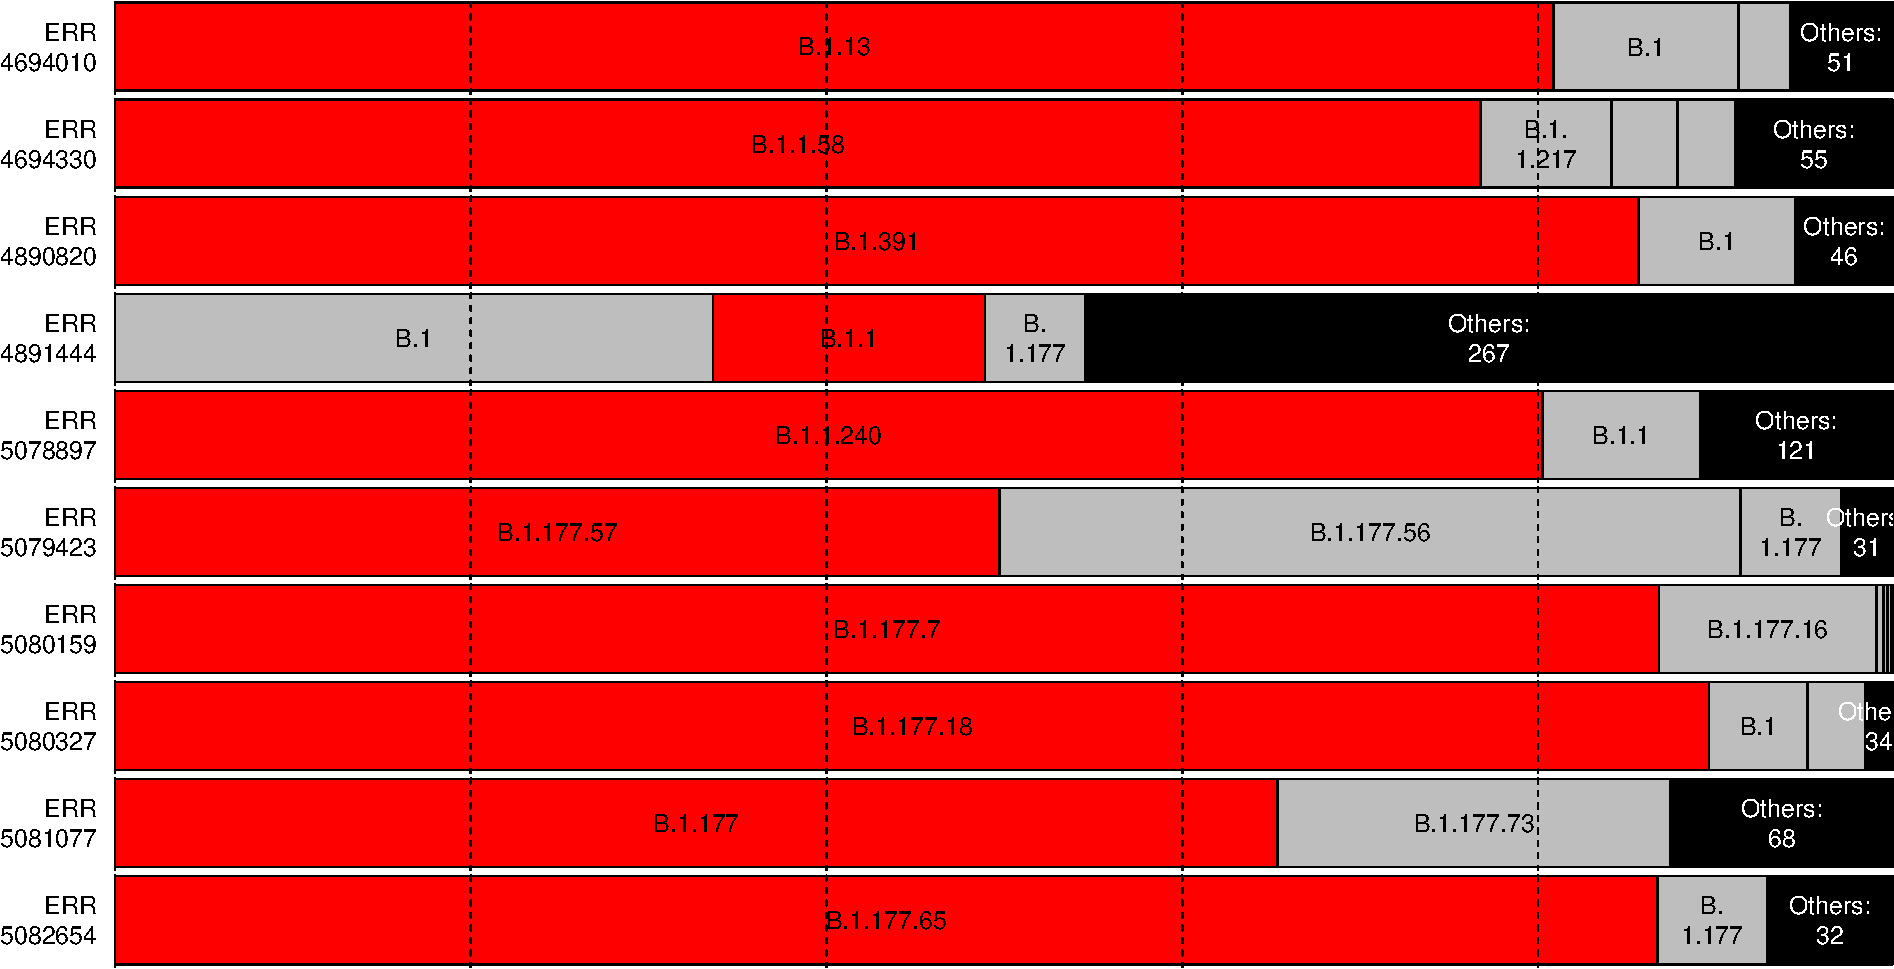
\includegraphics{pangolin_results_report_files/figure-latex/pareto-1.pdf}

\begin{Shaded}
\begin{Highlighting}[]
\NormalTok{seq\_info}\OperatorTok{$}\NormalTok{taxon \textless{}{-}}\StringTok{ }\NormalTok{taxons}
\NormalTok{seq\_info \textless{}{-}}\StringTok{ }\KeywordTok{arrange}\NormalTok{(seq\_info, mode, mode\_n) }\OperatorTok{\%\textgreater{}\%}
\StringTok{    }\KeywordTok{select}\NormalTok{(taxon, }\KeywordTok{everything}\NormalTok{())}
\NormalTok{knitr}\OperatorTok{::}\KeywordTok{kable}\NormalTok{(seq\_info, }\DataTypeTok{row.names =} \OtherTok{FALSE}\NormalTok{)}
\end{Highlighting}
\end{Shaded}

\begin{longtable}[]{@{}lllrrlrrr@{}}
\toprule
taxon & called & mode & mode\_n & perc & runner\_up & ru\_n & unique &
atoms\tabularnewline
\midrule
\endhead
SRR12762573 & A & A & 3532 & 70.68 & B & 1028 & 17 & 4\tabularnewline
SRR13092002 & A.1 & A.1 & 4922 & 98.50 & B.40 & 37 & 17 &
7\tabularnewline
SRR13020990 & A.2.2 & A.2.2 & 2892 & 57.87 & A.2 & 737 & 107 &
48\tabularnewline
ERR4891988 & B & B & 3914 & 78.33 & B.23 & 296 & 55 & 24\tabularnewline
ERR4999282 & B & B & 4041 & 80.87 & B.54 & 246 & 53 & 11\tabularnewline
ERR4891715 & B & B & 4521 & 90.47 & B.23 & 123 & 28 & 6\tabularnewline
SRR13020989 & B.1.1.273 & B.1 & 1338 & 26.87 & B & 302 & 425 &
132\tabularnewline
ERR4440194 & B.1 & B.1 & 2575 & 51.53 & B.1.98 & 2254 & 18 &
4\tabularnewline
ERR4891841 & B.1 & B.1 & 3785 & 75.75 & B.1.243 & 38 & 219 &
52\tabularnewline
ERR4890354 & B.1 & B.1 & 4326 & 86.57 & B.1.243 & 25 & 179 &
48\tabularnewline
ERR4893013 & B.1 & B.1 & 4444 & 88.93 & B.1.88 & 124 & 49 &
17\tabularnewline
ERR4692364 & B.1 & B.1 & 4524 & 90.53 & B.1.400 & 170 & 58 &
25\tabularnewline
ERR4440731 & B.1 & B.1 & 4666 & 93.38 & B.1.391 & 50 & 54 &
19\tabularnewline
ERR5069624 & B.1 & B.1 & 4821 & 96.48 & B.1.247 & 83 & 42 &
18\tabularnewline
ERR4694556 & B.1.1.15 & B.1.1.15 & 4772 & 95.50 & B.1.1.107 & 19 & 57 &
17\tabularnewline
ERR4892293 & B.1.1.162 & B.1.1.162 & 3145 & 62.94 & B.1.1.197 & 93 & 190
& 48\tabularnewline
ERR4440219 & B.1.1.164 & B.1.1.164 & 4682 & 93.70 & B.1.1 & 32 & 70 &
23\tabularnewline
ERR4891863 & B.1.1.216 & B.1.1.216 & 4201 & 84.07 & B.1 & 119 & 127 &
48\tabularnewline
ERR4893186 & B.1.1.216 & B.1.1.216 & 4432 & 88.69 & B.1 & 44 & 86 &
24\tabularnewline
ERR4892203 & B.1.1.216 & B.1.1.216 & 4495 & 89.95 & B.1.1.208 & 64 & 90
& 24\tabularnewline
ERR5080893 & B.1.1.251 & B.1.1.251 & 2943 & 58.90 & B.1 & 185 & 149 &
27\tabularnewline
ERR4664555 & B.1.1.253 & B.1.1.253 & 4813 & 96.32 & B.1 & 49 & 23 &
4\tabularnewline
ERR4307842 & B.1.1.289 & B.1.1.289 & 4745 & 94.96 & B.1 & 56 & 29 &
11\tabularnewline
ERR4759453 & B.1.1.29 & B.1.1.29 & 977 & 19.55 & B.1.1.208 & 244 & 207 &
47\tabularnewline
ERR4440425 & B.1.1.29 & B.1.1.29 & 1076 & 21.53 & B.1 & 129 & 260 &
24\tabularnewline
ERR4892066 & B.1.1.29 & B.1.1.29 & 1297 & 25.96 & B.1.1.59 & 343 & 231 &
56\tabularnewline
ERR4890228 & B.1.1.29 & B.1.1.29 & 1982 & 39.66 & B.1.1.273 & 133 & 232
& 58\tabularnewline
ERR4893037 & B.1.1.29 & B.1.1.29 & 2495 & 49.93 & B.1 & 90 & 223 &
28\tabularnewline
ERR4890294 & B.1.1.29 & B.1.1.29 & 2710 & 54.23 & B.1.1.37 & 521 & 189 &
41\tabularnewline
ERR4440247 & B.1.1.29 & B.1.1.29 & 3155 & 63.14 & B.1 & 229 & 227 &
38\tabularnewline
ERR4694571 & B.1.1.29 & B.1.1.29 & 3176 & 63.56 & B.1.1.44 & 131 & 213 &
42\tabularnewline
ERR4440354 & B.1.1.29 & B.1.1.29 & 3323 & 66.50 & B.1.1.132 & 65 & 211 &
33\tabularnewline
ERR4440402 & B.1.1.29 & B.1.1.29 & 3490 & 69.84 & B.1 & 168 & 215 &
45\tabularnewline
ERR4364007 & B.1.1.29 & B.1.1.29 & 4271 & 85.47 & B.1.1 & 56 & 89 &
29\tabularnewline
ERR4694617 & B.1.1.304 & B.1.1.304 & 4711 & 94.28 & B.1.1.10 & 66 & 28 &
3\tabularnewline
ERR4891898 & B.1.1.304 & B.1.1.304 & 4831 & 96.68 & B.1.1.4 & 18 & 29 &
7\tabularnewline
ERR4893033 & B.1.1.307 & B.1.1.307 & 4870 & 97.46 & B.1 & 63 & 34 &
22\tabularnewline
ERR5062514 & B.1.1.307 & B.1.1.307 & 4943 & 98.92 & B.1.1.311 & 18 & 17
& 10\tabularnewline
ERR4892048 & B.1.1.307 & B.1.1.307 & 4966 & 99.38 & B.1.1.311 & 16 & 8 &
5\tabularnewline
ERR4893353 & B.1.1.307 & B.1.1.307 & 4973 & 99.52 & B.1 & 13 & 7 &
3\tabularnewline
ERR4890271 & B.1.1.307 & B.1.1.307 & 4978 & 99.62 & B.1 & 7 & 8 &
3\tabularnewline
ERR4693079 & B.1.1.310 & B.1.1.310 & 4376 & 87.57 & B.1.1.29 & 231 & 107
& 50\tabularnewline
ERR4693034 & B.1.1.310 & B.1.1.310 & 4399 & 88.03 & B.1.1.59 & 57 & 89 &
44\tabularnewline
ERR5080913 & B.1.1.311 & B.1.1.311 & 4861 & 97.28 & B.1.1.281 & 47 & 16
& 8\tabularnewline
ERR5082696 & B.1.1.315 & B.1.1.315 & 4575 & 91.55 & B.1 & 147 & 43 &
20\tabularnewline
ERR5082664 & B.1.1.315 & B.1.1.315 & 4866 & 97.38 & B.1 & 60 & 13 &
4\tabularnewline
ERR4667618 & B.1.1.315 & B.1.1.315 & 4933 & 98.72 & B.1 & 30 & 11 &
3\tabularnewline
ERR4869497 & B.1.1.315 & B.1.1.315 & 4944 & 98.94 & B.1 & 15 & 11 &
4\tabularnewline
ERR5062388 & B.1.1.7 & B.1.1.7 & 4997 & 100.00 & NA & NA & 1 &
0\tabularnewline
ERR5062935 & B.1.1.7 & B.1.1.7 & 4997 & 100.00 & NA & NA & 1 &
0\tabularnewline
ERR5063143 & B.1.1.7 & B.1.1.7 & 4997 & 100.00 & NA & NA & 1 &
0\tabularnewline
ERR5063807 & B.1.1.7 & B.1.1.7 & 4997 & 100.00 & NA & NA & 1 &
0\tabularnewline
ERR5064346 & B.1.1.7 & B.1.1.7 & 4997 & 100.00 & NA & NA & 1 &
0\tabularnewline
ERR5064811 & B.1.1.7 & B.1.1.7 & 4997 & 100.00 & NA & NA & 1 &
0\tabularnewline
ERR5069584 & B.1.1.7 & B.1.1.7 & 4997 & 100.00 & NA & NA & 1 &
0\tabularnewline
ERR5069616 & B.1.1.7 & B.1.1.7 & 4997 & 100.00 & NA & NA & 1 &
0\tabularnewline
ERR5069871 & B.1.1.7 & B.1.1.7 & 4997 & 100.00 & NA & NA & 1 &
0\tabularnewline
ERR5070294 & B.1.1.7 & B.1.1.7 & 4997 & 100.00 & NA & NA & 1 &
0\tabularnewline
ERR5077411 & B.1.1.7 & B.1.1.7 & 4997 & 100.00 & NA & NA & 1 &
0\tabularnewline
ERR5077618 & B.1.1.7 & B.1.1.7 & 4997 & 100.00 & NA & NA & 1 &
0\tabularnewline
ERR5082610 & B.1.1.7 & B.1.1.7 & 4997 & 100.00 & NA & NA & 1 &
0\tabularnewline
ERR5074314 & B.1.160 & B.1.160 & 4833 & 96.72 & B.1.160.8 & 95 & 18 &
10\tabularnewline
ERR5082569 & B.1.160 & B.1.160 & 4845 & 96.96 & B.1.160.5 & 68 & 23 &
10\tabularnewline
ERR4869446 & B.1.160.7 & B.1.160.7 & 4947 & 99.00 & B.1.160 & 42 & 5 &
0\tabularnewline
ERR5082711 & B.1.177 & B.1.177 & 3683 & 73.70 & B.1.177.22 & 749 & 29 &
11\tabularnewline
ERR5082645 & B.1.177 & B.1.177 & 3805 & 76.15 & B.1.177.22 & 517 & 22 &
7\tabularnewline
ERR4893031 & B.1.177 & B.1.177 & 3812 & 76.29 & B.1.177.7 & 1003 & 19 &
7\tabularnewline
ERR4892152 & B.1.177 & B.1.177 & 4260 & 85.25 & B.1.177.7 & 498 & 14 &
3\tabularnewline
ERR5082561 & B.1.177 & B.1.177 & 4313 & 86.31 & B.1.177.22 & 447 & 22 &
5\tabularnewline
ERR5062062 & B.1.177 & B.1.177 & 4326 & 86.57 & B.1.177.8 & 381 & 16 &
2\tabularnewline
ERR5082695 & B.1.177 & B.1.177 & 4483 & 89.71 & B.1.177.22 & 297 & 19 &
4\tabularnewline
ERR4869480 & B.1.177 & B.1.177 & 4511 & 90.27 & B.1.177.22 & 252 & 22 &
5\tabularnewline
ERR4893242 & B.1.177 & B.1.177 & 4561 & 91.27 & B.1.177.6 & 164 & 15 &
3\tabularnewline
ERR4892339 & B.1.177 & B.1.177 & 4566 & 91.37 & B.1.177.23 & 131 & 19 &
1\tabularnewline
ERR5082576 & B.1.177 & B.1.177 & 4567 & 91.39 & B.1.177.22 & 237 & 20 &
1\tabularnewline
ERR5064294 & B.1.177 & B.1.177 & 4576 & 91.57 & B.1.177.27 & 272 & 14 &
2\tabularnewline
ERR5082580 & B.1.177 & B.1.177 & 4601 & 92.08 & B.1.177.22 & 242 & 20 &
1\tabularnewline
ERR5081301 & B.1.177 & B.1.177 & 4638 & 92.82 & B.1.177.22 & 195 & 21 &
4\tabularnewline
ERR4869458 & B.1.177 & B.1.177 & 4648 & 93.02 & B.1.177.22 & 198 & 19 &
3\tabularnewline
ERR4869487 & B.1.177 & B.1.177 & 4702 & 94.10 & B.1.177.22 & 147 & 17 &
1\tabularnewline
ERR5080918 & B.1.177 & B.1.177 & 4723 & 94.52 & B.1.177.22 & 150 & 19 &
4\tabularnewline
ERR5064166 & B.1.177 & B.1.177 & 4731 & 94.68 & B.1.177.22 & 149 & 16 &
1\tabularnewline
ERR5062729 & B.1.177 & B.1.177 & 4760 & 95.26 & B.1.177.22 & 116 & 14 &
1\tabularnewline
ERR4893080 & B.1.177 & B.1.177 & 4767 & 95.40 & B.1.177.22 & 118 & 14 &
5\tabularnewline
ERR5063922 & B.1.177 & B.1.177 & 4769 & 95.44 & B.1.177.22 & 148 & 16 &
1\tabularnewline
ERR4892392 & B.1.177 & B.1.177 & 4770 & 95.46 & B.1.177.22 & 95 & 18 &
5\tabularnewline
ERR5063539 & B.1.177 & B.1.177 & 4774 & 95.54 & B.1.177.22 & 121 & 20 &
4\tabularnewline
ERR4893197 & B.1.177 & B.1.177 & 4779 & 95.64 & B.1.177.23 & 105 & 18 &
5\tabularnewline
ERR5077151 & B.1.177 & B.1.177 & 4785 & 95.76 & B.1.177.22 & 114 & 20 &
2\tabularnewline
ERR5062571 & B.1.177 & B.1.177 & 4800 & 96.06 & B.1.177.22 & 98 & 21 &
3\tabularnewline
ERR5060778 & B.1.177 & B.1.177 & 4827 & 96.60 & B.1.177.22 & 115 & 15 &
5\tabularnewline
ERR4890403 & B.1.177 & B.1.177 & 4831 & 96.68 & B.1.177.22 & 82 & 18 &
5\tabularnewline
ERR5070060 & B.1.177 & B.1.177 & 4854 & 97.14 & B.1.177.22 & 69 & 14 &
2\tabularnewline
ERR5081316 & B.1.177.15 & B.1.177.15 & 4799 & 96.04 & B.1.177 & 131 & 16
& 6\tabularnewline
ERR4893138 & B.1.177.16 & B.1.177.16 & 4954 & 99.14 & B.1.177 & 30 & 7 &
3\tabularnewline
ERR4892200 & B.1.177.17 & B.1.177.17 & 4956 & 99.18 & B.1.177 & 39 & 4 &
2\tabularnewline
ERR5064787 & B.1.177.17 & B.1.177.17 & 4958 & 99.22 & B.1.177 & 23 & 5 &
2\tabularnewline
ERR4890386 & B.1.177.18 & B.1.177.18 & 4969 & 99.44 & B.1.177.13 & 15 &
6 & 2\tabularnewline
ERR5076163 & B.1.177.19 & B.1.177.19 & 4856 & 97.18 & B.1.177 & 99 & 11
& 1\tabularnewline
ERR5076748 & B.1.177.19 & B.1.177.19 & 4892 & 97.90 & B.1.177 & 67 & 12
& 5\tabularnewline
ERR5063165 & B.1.177.19 & B.1.177.19 & 4905 & 98.16 & B.1.177 & 67 & 8 &
2\tabularnewline
ERR5063813 & B.1.177.19 & B.1.177.19 & 4932 & 98.70 & B.1.177 & 47 & 9 &
3\tabularnewline
ERR4693605 & B.1.177.3 & B.1.177.3 & 4825 & 96.56 & B.1.177 & 68 & 17 &
2\tabularnewline
ERR5081304 & B.1.177.4 & B.1.177.4 & 4954 & 99.14 & B.1.177.2 & 21 & 17
& 10\tabularnewline
ERR5082590 & B.1.177.4 & B.1.177.4 & 4971 & 99.48 & B.1.177.2 & 13 & 11
& 7\tabularnewline
ERR5062648 & B.1.177.4 & B.1.177.4 & 4988 & 99.82 & B.1.177 & 4 & 6 &
3\tabularnewline
ERR5082674 & B.1.177.6 & B.1.177.6 & 4858 & 97.22 & B.1.177 & 79 & 13 &
4\tabularnewline
ERR4891805 & B.1.177.6 & B.1.177.6 & 4939 & 98.84 & B.1.177 & 24 & 8 &
0\tabularnewline
ERR5082712 & B.1.177.7 & B.1.177.7 & 3334 & 66.72 & B.1.177 & 1612 & 15
& 5\tabularnewline
ERR5082556 & B.1.177.7 & B.1.177.7 & 3766 & 75.37 & B.1.177 & 1195 & 11
& 2\tabularnewline
ERR5082630 & B.1.177.7 & B.1.177.7 & 4833 & 96.72 & B.1.177 & 128 & 13 &
6\tabularnewline
ERR4693537 & B.1.177.7 & B.1.177.7 & 4849 & 97.04 & B.1.177 & 126 & 13 &
6\tabularnewline
ERR4363387 & B.1.222 & B.1.222 & 4761 & 95.28 & B.1 & 96 & 27 &
14\tabularnewline
ERR5081322 & B.1.235 & B.1.235 & 4743 & 94.92 & B.1 & 128 & 21 &
8\tabularnewline
ERR4893184 & B.1.258 & B.1.258 & 4099 & 82.03 & B.1.258.17 & 435 & 35 &
15\tabularnewline
ERR5062004 & B.1.258 & B.1.258 & 4563 & 91.31 & B.1 & 80 & 35 &
7\tabularnewline
ERR4891711 & B.1.36 & B.1.36 & 4770 & 95.46 & B.1.36.9 & 81 & 27 &
8\tabularnewline
ERR4890371 & B.1.36.17 & B.1.36.17 & 4177 & 83.59 & B.1 & 491 & 45 &
17\tabularnewline
ERR5080897 & B.1.36.17 & B.1.36.17 & 4763 & 95.32 & B.1 & 132 & 24 &
13\tabularnewline
ERR4890352 & B.1.36.17 & B.1.36.17 & 4938 & 98.82 & B.1 & 20 & 16 &
10\tabularnewline
ERR4890337 & B.1.36.17 & B.1.36.17 & 4951 & 99.08 & B.1 & 20 & 9 &
3\tabularnewline
ERR4892423 & B.1.523 & B.1.523 & 4493 & 89.91 & B.1 & 128 & 31 &
9\tabularnewline
ERR4893393 & B.1.523 & B.1.523 & 4658 & 93.22 & B.1 & 153 & 36 &
15\tabularnewline
ERR4890285 & B.1.523 & B.1.523 & 4892 & 97.90 & B.1 & 50 & 23 &
9\tabularnewline
ERR4891889 & B.1.98 & B.1.98 & 4166 & 83.37 & B.1 & 311 & 70 &
42\tabularnewline
ERR4693061 & B.23 & B.23 & 4734 & 94.74 & B.48 & 113 & 19 &
5\tabularnewline
ERR4694400 & B.3 & B.3 & 4903 & 98.12 & B.3.1 & 42 & 13 &
3\tabularnewline
ERR4305816 & B.3.1 & B.3.1 & 4788 & 95.82 & B.3 & 147 & 15 &
3\tabularnewline
ERR4892112 & B.39 & B.39 & 4733 & 94.72 & B.3 & 85 & 31 &
13\tabularnewline
ERR4890427 & B.39 & B.39 & 4757 & 95.20 & A.16 & 96 & 20 &
4\tabularnewline
ERR4440332 & B.40 & B.40 & 4917 & 98.40 & B.1 & 41 & 8 &
2\tabularnewline
ERR4892386 & B.40 & B.40 & 4967 & 99.40 & B.1 & 10 & 8 &
2\tabularnewline
ERR4440373 & B.40 & B.40 & 4972 & 99.50 & B & 10 & 9 & 5\tabularnewline
ERR4891916 & None & None & 4993 & 99.96 & B.1 & 2 & 2 & 0\tabularnewline
ERR4999251 & None & None & 4997 & 100.00 & NA & NA & 1 &
0\tabularnewline
ERR4999255 & None & None & 4997 & 100.00 & NA & NA & 1 &
0\tabularnewline
ERR4999275 & None & None & 4997 & 100.00 & NA & NA & 1 &
0\tabularnewline
SRR12639958 & None & None & 4997 & 100.00 & NA & NA & 1 &
0\tabularnewline
\bottomrule
\end{longtable}

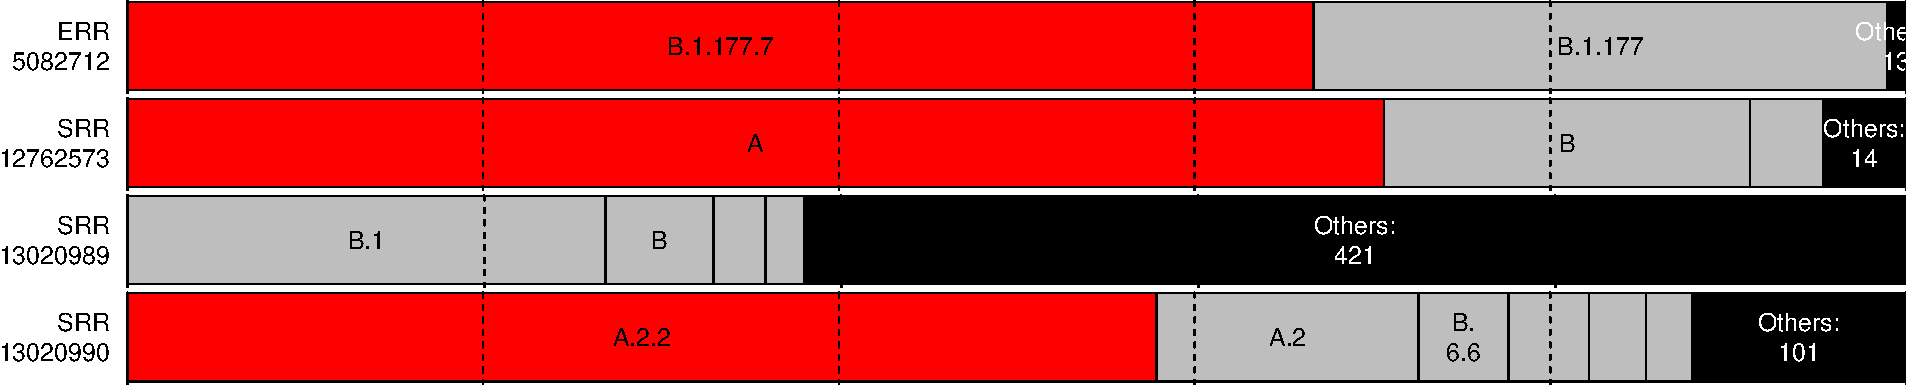
\includegraphics{pangolin_results_report_files/figure-latex/pareto-2.pdf}

\end{document}
